\section{Method}
\label{sec:method}

Each item $i$ has a score $s_i$.
The probability that $i$ beats $j$ is $\sigma(s_i - s_j)$, as in standard paired comparison models~\cite{Hunter2004}.
We fit the scores by maximum likelihood and measure fitness as the share of outcomes the fitted order predicts.
Figure~\ref{fig:one} shows the score distribution.

\begin{figure}[t]
  \centering
  % ploma:source scripts/make_fig1.py --season 2023
  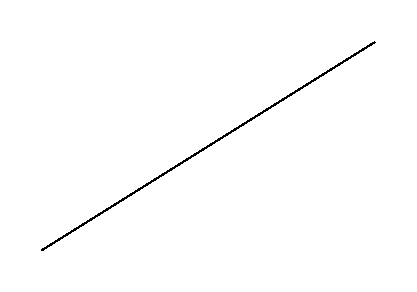
\includegraphics[width=0.6\linewidth]{figures/fig1.pdf}
  \caption{Fitted scores for all items.}
  \label{fig:one}
\end{figure}
